\chapter{Choosing an Implementation Approach}

\section{Viability of a Slurm Plugin}
\label{subsec:slurm_plugin}

Our first idea was to use a non-simulation approach. 
The HPI's Data Lab\webcite{web_delabhpi} runs a \emph{Slurm} cluster and also has some nodes with power measurement infrastructure included. 
Slurm is an "open-source, fault-tolerant, and highly scalable cluster management and job scheduling system for large and small Linux clusters".\webcite{web_slurm}
The job scheduling part is important here, it also supports a plugin infrastructure that includes scheduling plugins. 
One of the highlighted papers\cite{inigo_goiri_greenslot_2011} in the related work section specifically used Slurm for its carbon-aware scheduler implementation and thus seemed like a good starting point for our work.

\paragraph{Installing Slurm locally}

For our purposes, a local installation suffices as we do not need to run heavy workloads but instead only need the scheduling part of Slurm. 
While there is a Slurm \verb|apt get| package for Ubuntu, extending this with plugins is not possible as plugins need to be included during the Slurm compilation, meaning we will have to do the same.

Slurm's documentation provides some guidelines on how to install Slurm, which we followed. 
We tried cloning the main branch, but the compilation process encountered an error midway. However, using the predefined released versions worked.
Installing \verb|munge|\webcite{web_munge} is also necessary, which is used for authentication in Slurm.

One problem arose as we tried to start the \verb|Slurmd|- and \verb|Slurmctld| services. The first one is the worker service that later executes jobs submitted to Slurm. The latter is the main controller that, for example, schedules jobs on workers. While the command to start them did not fail, upon node inspection via Slurm's \verb|scontrol| command, it showed that all nodes were \verb|DOWN| instantly.

Dealing with Slurm's problems usually leads to inspecting its logs, in this case, the logs showed the following:

\begin{minipage}{\linewidth}
\begin{lstlisting}[language=bash, frame=single, numbers=none, caption={Slurm's cgroup configuration is missing according to the logs}, basicstyle=\ttfamily]
$ less config.log

error: Couldn't find the specified plugin name for cgroup/v2
    looking at all files
error: cannot find cgroup plugin for cgroup/v2
error: cannot create cgroup context for cgroup/v2
error: Unable to initialize cgroup plugin
error: Slurmd initialization failed
\end{lstlisting}
\end{minipage}

Slurm uses Linux's \verb|cgroup| feature to manage the submitted job's hardware resources. The log hints at some problems related to Slurm's usage of it.
The solution was to provide Slurm's \verb|cgroup.conf| file. In our use-case of getting Slurm to simply start, this did not need to be very sophisticated, so we just used an off-the-shelf configuration file.\webcite{web_slurmd}
Running \verb|scontrol| again, we were now able to see idling nodes, meaning that Slurm was successfully installed from source.

\paragraph{Creating a Scheduler Plugin}

The Slurm documentation provides a short guide on how to add a plugin to Slurm.\webcite{web_slurmguide}
As a start, we simply copied Slurm's default scheduler (which is also a plugin) to the specified directory under a new name, and added that new name to Slurms build files. 
It was then time to recompile Slurm. 
Now, however, during the recommended \verb|autoreconf| step, an error occurred:

\begin{minipage}{\linewidth}
\begin{lstlisting}[language=bash, frame=single, numbers=none, caption={Plugin recompilation errors}, basicstyle=\ttfamily]
$ autoreconf
auxdir/x_ac_sview.m4:35: warning: macro 'AM_PATH_GLIB_2_0' 
    not found in library
configure:25140: error: possibly undefined macro: AM_PATH_GLIB_2_0
      If this token and others are legitimate, 
      please use m4_pattern_allow.
      See the Autoconf documentation.
autoreconf: error: /usr/bin/autoconf failed with exit status: 1
\end{lstlisting}
\end{minipage}

The solution, while not very obvious, was to install the \verb|libgtk2.0-dev| library\webcite{web_slurmsim}.
We then added a simple logging to the new plugin. Upon inspecting the logs after scheduling a hello-world-script, that log message showed up as well - confirming that our new scheduler plugin was running.

\paragraph{Adding more logic to the scheduler plugin}

One very helpful step for developing inside Slurm is to enable the debugging flags.
This must be decided before compilation by using the \verb|--enable-developer| and \verb|--disable-optimizations| flags during the \verb|/configure| step. 
With that, debug symbols are added to the outgoing binaries. 
As we were using VS Code, we could then attach its debugger to the running Slurm thread with full functionality.

The code of the plugin runs in its own thread and there is no sandboxing or similar around it.
Thus, there are seemingly no limitations on what can be done inside the plugin. 
For testing, we read information on the incoming jobs such as set constraints or the user-supplied comments. Terminating the jobs was also possible inside the plugin.

\paragraph{Problems of a scheduler plugin}

One big problem manifested in that not all jobs \emph{showed up} inside the plugin's job queue. 
If we submitted 6 jobs, via Slurm's \verb|squeue| command, only a part, such as the last 3, logged inside the plugin.
A possible explanation for this could be Slurms' scheduler architecture: while there is a scheduler plugin, there also is a scheduler inside Slurm's main loop. These both work in parallel\webcite{web_slurmsourcecode} and they use the same job queue.

To hack around this, we tried disabling Slurm's main scheduling loop by setting \verb|sched_interval=-1| inside the Slurm configuration file. 
While this had the effect of being able to access all incoming jobs inside the plugin, it also had the side effect of disabling all logic concerning starting the jobs.
So by choosing this route, the plugin needs to re-implement a lot of extra logic, which conventionally is not inside the scheduler plugin. 

We also looked into whether there were any API hooks that are exposed to the plugin. 
Up until Slurm version 20.11, scheduler plugins had callbacks\webcite{web_slurm_plugin_old} such as a job just getting submitted. There also was support for \emph{passive} schedulers that were invoked when determined by Slurm.
The version we used, however,  23.11, removed all such functionality and documentation.\webcite{web_slurm_plugin_current} All plugins are implemented via threads that only have callbacks for when they are started and stopped.

Thus, since there was no apparent way of getting around this scheduler race condition between the plugin and the main loop, the scheduler approach was dropped. 
While we would not say that a plugin approach is impossible, the effort to implement one from scratch seems very high. 
The public documentation for developing Slurm is scarce. 
There is a mailing list that can be searched, but it looks to be mostly aimed at administrating Slurm and not developing it.

Other avenues that could be explored are Slurm's Lua plugins. 
There is also a \emph{Slurm simulator}\webcite{web_slurmsim} which could potentially be used for carbon-aware scheduling simulation, but that we did not look into much for reasons of little documentation and a seeming lack of continued support.

\section{Simulating with \programname{}}

\paragraph{Description of the GAIA Simulator}

We first describe the existing testbed and make it clear which part is our work and which is not. A class diagram is provided in \ref{fig:class_diagram} which is heavily inspired by the existing architecture diagram in the original paper. 

\begin{figure}
    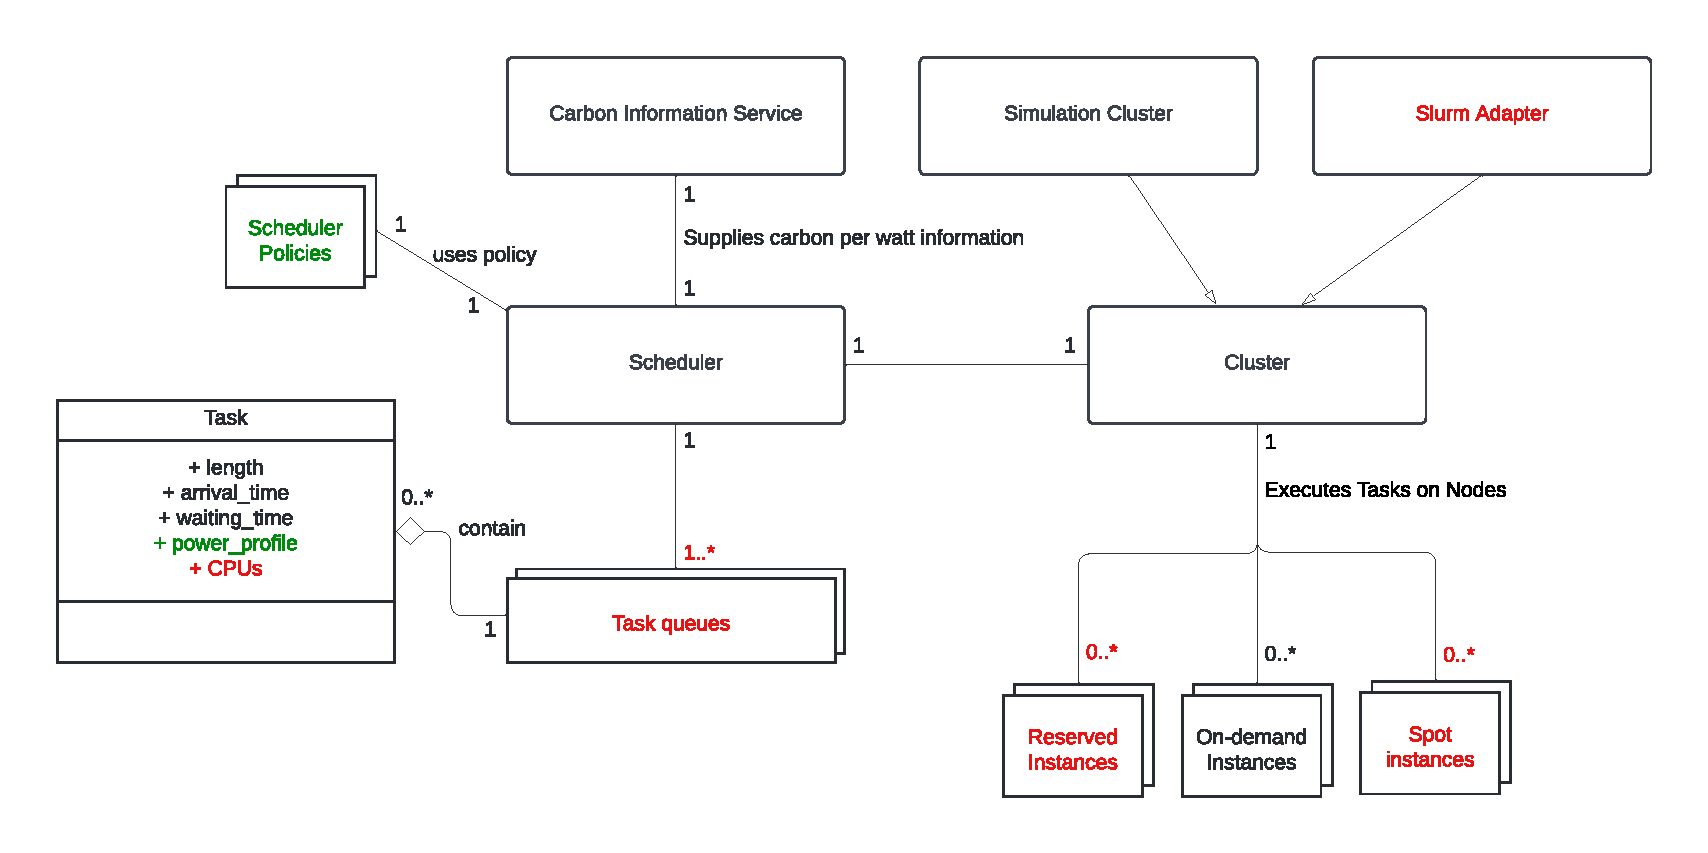
\includegraphics[width=\linewidth]{images/MA Thesis Diagram.pdf}
    \caption{Class diagram of \programname{}, which is a fork of GAIA (black). Green indicates addition. Red indicates removal of the original GAIA features.}
    \label{fig:class_diagram}
\end{figure}

The main part of GAIA is the scheduler. At program start, it takes parameters\todo{I should probably give an overview of which parameters are supported, so I have that terminology later} that determine the scheduling, such as whether tasks can be interrupted, how to use the carbon information (e.g. use a perfect-information / oracle approach or use a running average), and how to balance the dollar cost of scheduling. 
The latter we removed for simplicity, which is marked in the figure via the red color of the reserved and spot instances. In our case of carbon-aware scheduling, we did not need that feature.

In the original implementation, the scheduler had multiple queues of tasks. 
The paper presented an approach of a short queue (tasks under 2 hours) and long tasks (all other), short tasks are scheduled on spot instances. 
Again, as we already removed the spot instance, feature, the queue multiplicity was removed likewise.

The task queues are based on historical traces. GAIA provided multiple traces that are described in the paper.

Tasks have a predetermined length, as saved in the trace, and they also hold some data that is used for scheduling such as their arrival time in the system, and how long they should wait until execution. 
Some properties such as required CPUs were removed.
Our contribution of the phases-and-power model was added to the tasks.

The Scheduler policies are also marked green, as we added scheduler policies that could use \modelname. Specifically, we added a (non-) suspend \& resume scheduler that works on the assumption of perfect carbon intensity knowledge, this will be further explained in the latter sections.

Scheduled tasks are submitted to a cluster.
In our case, this is a simulated, already implemented, cluster that simply logs when each task is entered and finished. 
In the original paper, they also used an open-source adapter that submits the tasks to an actual Slurm cluster. 
While this approach could have been used, we decided against it based on not adding further complexity. 
Thus, we also removed the Slurm adapter from our implementation.

\chapter{Schedulers with \modelname{}}

We will first summarize the assumptions that GAIA makes on the problem of carbon-aware scheduling:

\begin{enumerate}
    \item job lengths are known
    \item all considered jobs are batch jobs and can thus be shifted temporally based on user deadlines
    \item carbon information is provided for near future periods, no error is considered
    \item there are no hardware limitations or considerations, all jobs are executed in an isolated manner
    \item jobs have a constant power draw and can be suspended \& resumed for free
\end{enumerate}

Especially the last point will be modified going further. As shown in Section \ref{sec:improving_the_model}, jobs now have a predefined, variable power draw according to the defined phases. Resuming a job will also carry an additional startup phase with it.

\section{Using \modelname{} in \programname{}}

The first step to be taken was to add the described model to the jobs as outlined in Figure \ref{fig:class_diagram}. 
So far, jobs were generated from \verb|csv|-formatted traces, one example being provided in Listing \ref{list:trace_csv}.

\begin{minipage}{\linewidth}
\begin{lstlisting}[frame=single, numbers=none, caption={Excerpt from the Alibaba-PAI trace}, label={list:trace_csv}, basicstyle=\ttfamily]
arrival_time,   length,     cpus
0.0,            6302.0,     1
68.0,           1000.0,     1
463.0,          1570.0,     3
838.0,          23549.0,    1
\end{lstlisting}
\end{minipage}

In the original GAIA implementation, jobs have an \verb|arrival_time|, which signifies when the job is added to the simulation in seconds. 
The \verb|length| of a job similarly encodes the seconds a job needs to fully execute. The \verb|cpu| column was not interesting for our work, as previously discussed.

The chosen way of supplying the model information was to add two new columns to the trace files, which entail the type of job and a column for arguments. 
As of now, the following types are supported: \verb|constant|, \verb|constant-from-phases|, \verb|phases|, and \verb|ml|. 
The first two \verb|constant| types are for backward compatibility with GAIA, and are for the evaluation later.

Type \verb|phases| is the main way of creating a job with phases such as the one used in the experiment. The supplied argument in that case would entail a Python-readable \verb|dict|, essentially a \verb|JSON|-like definition of the model as described in Listing \ref{listing:model_python}.
As this was just a string, we then used Python's \verb|eval()| to read it back into a Python object.\todo{Check how and if I should visualize this}
As an example, a simplified \verb|roberta.py|, the job that was measured in section \ref{sec:power_measurements}, could look like the code in Listing \ref{list:roberta_model_definition}

\begin{minipage}{\linewidth}
\begin{lstlisting}[frame=single, numbers=none, caption={Simplified definition for a job similar to the experiment}, label={list:roberta_model_definition}, basicstyle=\ttfamily]
{
    'startup': [
        {'name': 'Start', 'duration': 5.34, 'power': 59.9},
        {'name': 'Finish Imports', 'duration': 12.36, 'power': 53.77},
        {'name': 'Data loaded', 'duration': 5.75, 'power': 63.17}, 
    ],
    'work': [
        {'name': 'Train', 'duration': 8.17, 'power': 221.93}, 
        {'name': 'Evaluate', 'duration': 1.54, 'power': 134.0}, 
        {'name': 'Save', 'duration': 2.72, 'power': 105.1,
            'is_checkpoint': True}, 
    ] * 5
}
\end{lstlisting}
\end{minipage}

Instead of supplying the phase information via \verb|.csv|, we also added a parameter to set a value for all jobs.

To use \modelname{} and read out the power of a job at a given time, a function was created that essentially traverses all phases in order, keeping track of the time, and returning the power of the phase when the requested time is reached. 
This was also used to create Figure \ref{fig:model_overlaid}.

A generalizing helper type is \verb|ml|, which takes a dictionary of parameters and converts that to model parameters for the \verb|phases| type. A similar job as to the one above would be created with the following:

\begin{minipage}{\linewidth}
\begin{lstlisting}[frame=single, numbers=none, caption={Generic model definition for machine learning jobs}, label={list:roberta_model_definition_generic}, basicstyle=\ttfamily]
{
    'start_duration': 23.45
    'start_power': 60
    'training_duration': 8.17
    'training_power': 221.93
    'evaluate_duration': 1.54
    'evaluate_power': 63.17
    'save_duration': 2.72
    'save_power': 105.1
    'epochs': 5
}
\end{lstlisting}
\end{minipage}

\section{Uninterrupted oracle scheduling} \label{sec:uninterrupted_oracle_scheduling}

There already was an existing version of this scheduling approach which assumed constant power and that the carbon trace is fully known ("oracle"). 
Jobs is not able to suspend \& resume in this version.
The algorithm for which is pseudocoded in Listing \ref{list:pseudocode_oracle}.

\begin{minipage}{\linewidth}
\begin{lstlisting}[frame=single, numbers=left, caption={Pseudocode for the original non-interrupt oracle scheduler}, label={list:pseudocode_oracle}, basicstyle=\ttfamily]
function schedule_job_no_checkpointing_resuming(job):
    possible_starts = []
    for every possible starttime with respect to deadline:
        calculate carbon_emissions_of_job at starttime
        add carbon_emission, starttime to possible_starts
    
    return starttime with least carbon emissions

function carbon_emissions_of_job(job, carbon_trace):
    sum_of_emissions = 0

    for each second of job:
        sum_of_emissions += carbon_trace at timepoint * constant_watt
    
    return sum_of_emissions
\end{lstlisting}
\end{minipage}

In order to adjust this to \modelname, where power is a function of time, only line 13 needed changes. 
Thus, the previously mentioned time-to-power function replaced the Watt constant.
Evaluating this scheduling approach will take place in Section \ref{sec:evaluate_scheduling}, after another scheduling algorithm is introduced.

\section{{Suspend \& Resume Scheduling for Heterogeneous Jobs}} \label{sec:checkpoint_resume_lp}

Under the constant-power, no startup-overhead assumption of GAIA, the algorithm worked like the following:

\begin{enumerate}
    \item order all time slots until the deadline by their emissions ascending
    \item execute the job on the first length many time slots
\end{enumerate}

This minimizes emitted carbon, as only the best time slots are used.
Due to the diurnal nature of carbon emissions, this essentially uses each \emph{valley}, scheduling a job there. 
With deadlines increasing, the amount of suspends \& resumes also increases accordingly.

In order to implement a scheduler for the improved job model, we chose to use \emph{linear programming (LP)}.
In a nutshell, LP is an optimization method, that given linear equations and constraints, finds a set of variables (or a vector) that minimize (or maximize) an optimization goal.
Translating this to the context of carbon-aware scheduling, the resulting vector somehow decodes when a job should be executed.
The optimization goal in this case is to minimize the emitted carbon. 
A constraint for example could be that all time slots being executed should add up to the job length. 
The big challenge is then to model all of this in the form of mathematical equations, which will be most of this section's remainder.

\paragraph{Reflections on Linear Programming}

Linear programming is its own programming paradigm. Unlike, for example, imperative programming, where each instruction is coded explicitly, enabling classic debugging and such, in LP, a mathematical model is written which is then solved by a \emph{solver}. 
Different implementations for these solvers exist, but at least in our case, the result output by a solver will either be an error, or the result set. 
As the solver uses the whole model simultaneously, \emph{debugging} individual parts of the model is not possible outside of removing them from the overall model.

Thus, an iterative approach to LP proved useful. 
We encode some part of our overall problem into the model, solve it, and immediately plot the variables of the result set and check them visually.
The visual check is very important: many times the solver solved the problem "so well" that jobs are scheduled in a way that the emitted carbon is minimized, but the jobs are executed in edge cases that were not intended, but that are possible under the model, examples of this will be given in the following parts.

Another part of programming LP is \emph{just knowing the tricks}. 
Many common programming operations, especially ones for control flow, cannot be expressed directly (as they need to be a linear equation).
There are some mappings for such operations, but finding out how seems to be harder than in other paradigms, since the LP community appears to be smaller in comparison and online resources are limited.
Some \emph{tricks} will be highlighted in the latter parts as well. 

\paragraph{Modelling carbon-aware scheduling in a linear program}

In this part, we will present the iterative steps taken to model the scheduler as an LP problem, highlight some implementation details and visualize the results of each step.
We used Python's \verb|PuLP| library, which allows creating LP models to standard file types and also helps in calling external solvers as well as querying the results.

\paragraph{Executing the job}

Firstly, as the job has a certain length and a set deadline, we chose to use an array of time slot variables for the result set. Each such variable is a boolean signifying whether the job is executed at that time.
For the first constraint, the sum of all boolean variables (which are represented as 0 and 1) should add up to the job length, effectively executing the job for length-many time slots.
The necessary objective function is to be defined as each time slot being executed multiplied by the carbon-per-watt at that time slot.
As an example, the code for this is shown in Listing \ref{fig:lp_work}.

\begin{minipage}{\linewidth}
\begin{lstlisting}[frame=single, numbers=left, caption={LP Implementation for basic scheduling}, label={list:lp_work}, basicstyle=\ttfamily, breaklines]
prob = LpProblem("CarbonAwareScheduling", pulp.LpMinimize)
work = LpVariable.dicts("work", (t for t in range(DEADLINE)), cat="Binary")

prob += lpSum([work[t] * carbon_cost[t] for t in range(DEADLINE)]) 
prob += lpSum(work[t] for t in range(DEADLINE)) == WORK_LENGTH 

solver = pulp.Gurobi_CMD(timeLimit=timelimit)
prob.solve(solver)
\end{lstlisting}
\end{minipage}

\todo[inline]{Fix the stupid breaklines here}
The first line creates an LP problem and defines the optimization goal to be a minimizing one. 
Then, a variable "work" is defined as being \verb|DEADLINE|-many (in this case 300) integer-indexed boolean variables. 
These will be modeled as the time slots.
Line 4 defines the optimization goal; each time slot will be multiplied by the carbon emitted there. As one factor is a boolean, this will only increase the sum if the time slot is scheduled. The dictionary \verb|carbon_cost| contains a constant factor for each time slot.
The last two lines start the solving library. 
\verb|PuLP| offers an open-source solver by default, but during development this proved to be very slow and also did not offer features such as time limits and retrieving intermediate results.
We thus chose the \emph{Gurobi} solver, a commercial solver that also offers academic licenses. 
That one supported the previously lamented features and increased development time by a lot. 

The running example will be a deadline of 300 time slots, the job has a startup phase of 20 units and has 100 work units. 
The above code leads to a result set that is visualized in Figure \ref{fig:lp_work},
which on the bottom part shows the carbon emissions at each time slot and the upper graph shows the chosen time slots.
Looking at the figure, the results are not too surprising: the chosen time slots are just the points where emissions are lowest, essentially being equal to the result of the WaitAWhile-Algorithm.

\begin{figure}
    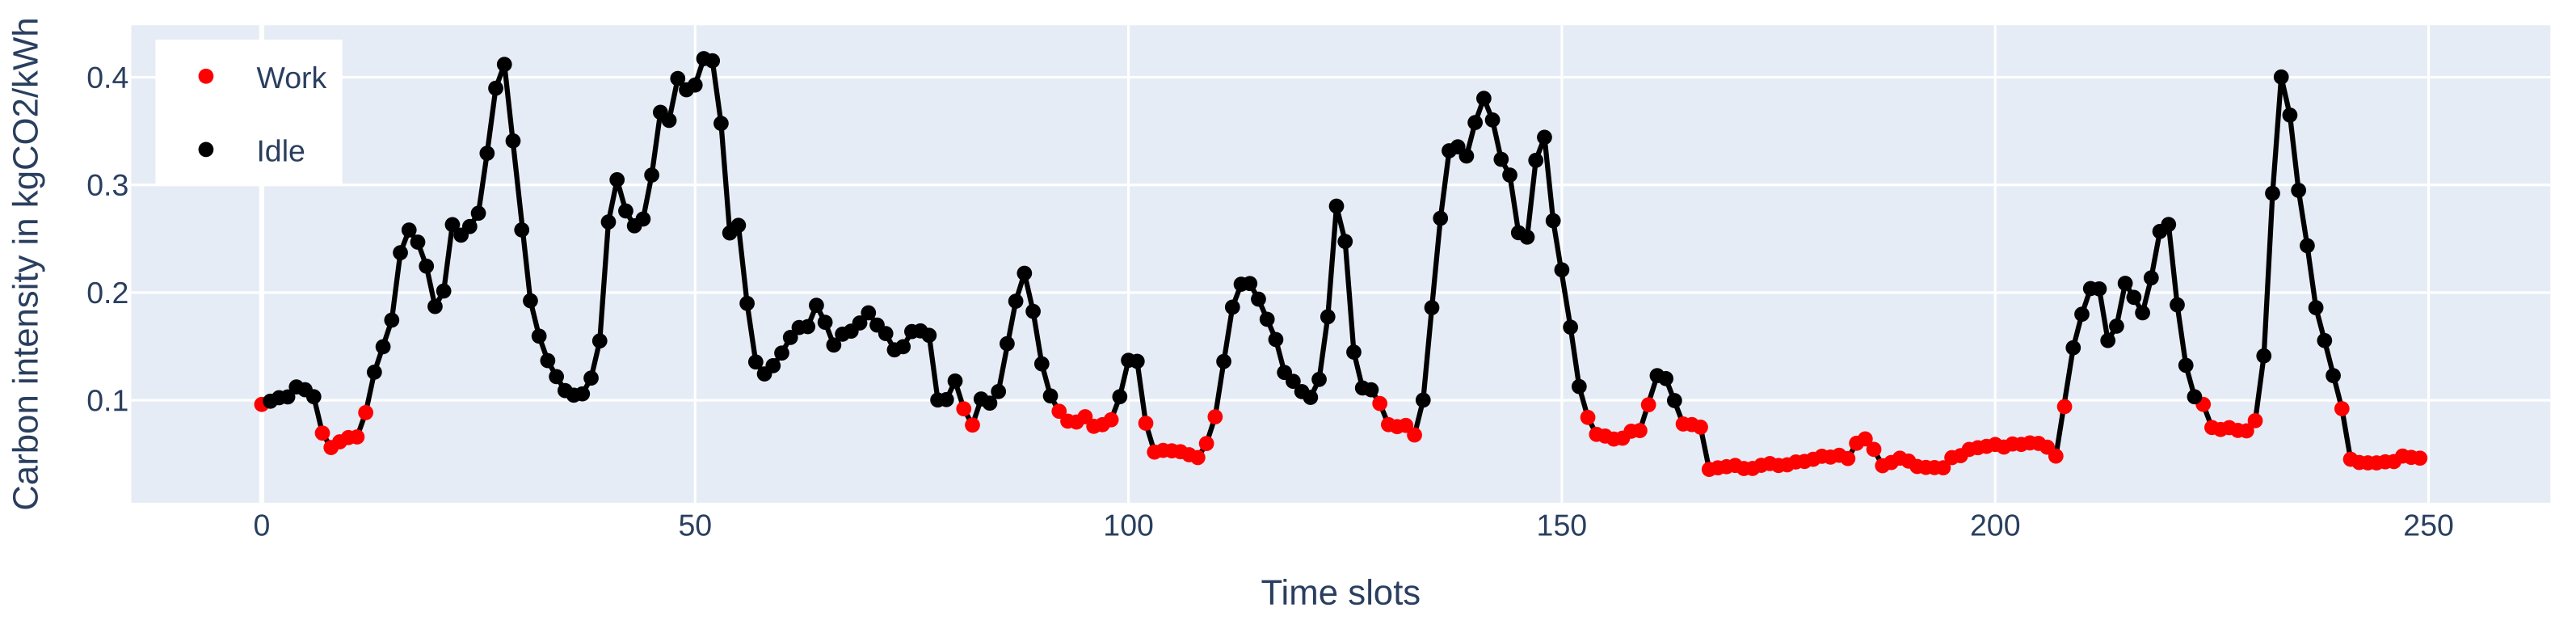
\includegraphics[width=\linewidth]{GAIA/notebooks/lp_work.pdf}
    \caption{Resulting schedule using the first iteration of the LP scheduler. Each time slot, with its corresponding carbon intensity, is assigned to be worked or not. As this iteration has no notion of startup-costs, only the lowest time slots are used with many suspends in between.}
    \label{fig:lp_work}
\end{figure}    

\paragraph{Adding Overhead via Startup Phases}

In order to add a cost to starting a job, the code following in listing \ref{list:lp_overhead} is complemented, some parts are excluded for brevity.

\begin{minipage}{\linewidth} % holy moly, hat er nicht gemacht 😏 tex.stackexchange.com/questions/73231/avoid-page-breaks-in-lstlistings
\begin{lstlisting}[frame=single, numbers=left, caption={LP Implementation for overhead}, label={list:lp_overhead}, basicstyle=\ttfamily]
for t in range(DEADLINE - 1):
    prob += startup_finished[t] >= work[t + 1] - work[t]
    prob += startup_finished[t] + work[t] <= 1
    prob += starting[t] + work[t] <= 1

for i in range(STARTUP_LENGTH - 1, DEADLINE):
    prob += pulp.lpSum([starting[i - j] for j in range(STARTUP_LENGTH)]) 
        >= STARTUP_LENGTH * startup_finished[i]
\end{lstlisting}
\end{minipage}


In this snippet, two extra dictionary variables are introduced, \verb|startup| and \verb|startup_finished|.
For every time slot (line 1), set \verb|startup_finished| to true if and only if there is a 0 to 1 transition along the \verb|work| dictionary (line 2). This becomes apparent when looking at Table \ref{tab:truth_table_startup_finished}.
Notice how the numerical booleans help in this case, as negative integers get mapped to \verb|0|, or \verb|false| respectively.

\begin{table}[h!]
\centering
\begin{tabular}{|c|c|c|c|}
\hline
    $work[t]$ & $work[t+1]$ & $work[t+1]$ - $work[t]$ & $startup\_finished[t]$ \\ \hline
    $0$ & $0$ & $0$ & $0$ \\ \hline
    $0$ & $1$ & $1$ & $1$ \\ \hline
    $1$ & $0$ & $max(-1, 0) = 0$ & $0$ \\ \hline
    $1$ & $1$ & $0$ & $0$ \\ \hline
\end{tabular}
\caption{Truth table for finding when working time slots begin}
\label{tab:truth_table_startup_finished}
\end{table}

Line 3 and 4 ensure that \emph{working} time slots and \emph{startup} time slots are mutually exclusive.
The last loop defines that if (\verb|* startup_finsihed[i]|) a startup must be finished by some time slot, the previous \verb|STARTUP_LENGTH|-many time slots must be used for starting the job.

At this point, sometimes, the solver scheduled jobs are set up at the very first time slots, as no startup could happen before time slot $0$, thus minimizing carbon but obviously producing a bogus result.
To fix this, we add an extra constraint that work may only be scheduled after the length of the startup phase.
The emitted carbon goal is changed to also include these new startup time slot, similarly to the previous Listing \ref{list:lp_overhead}.
With this step, the result already looks more like a reasonable schedule, as shown in Figure \ref{fig:lp_overhead}. 
This time, the optimal schedule includes executing the job in one go.
Doing a visual check, the job is also executed on seemingly the lowest carbon intensities.

\begin{figure}
    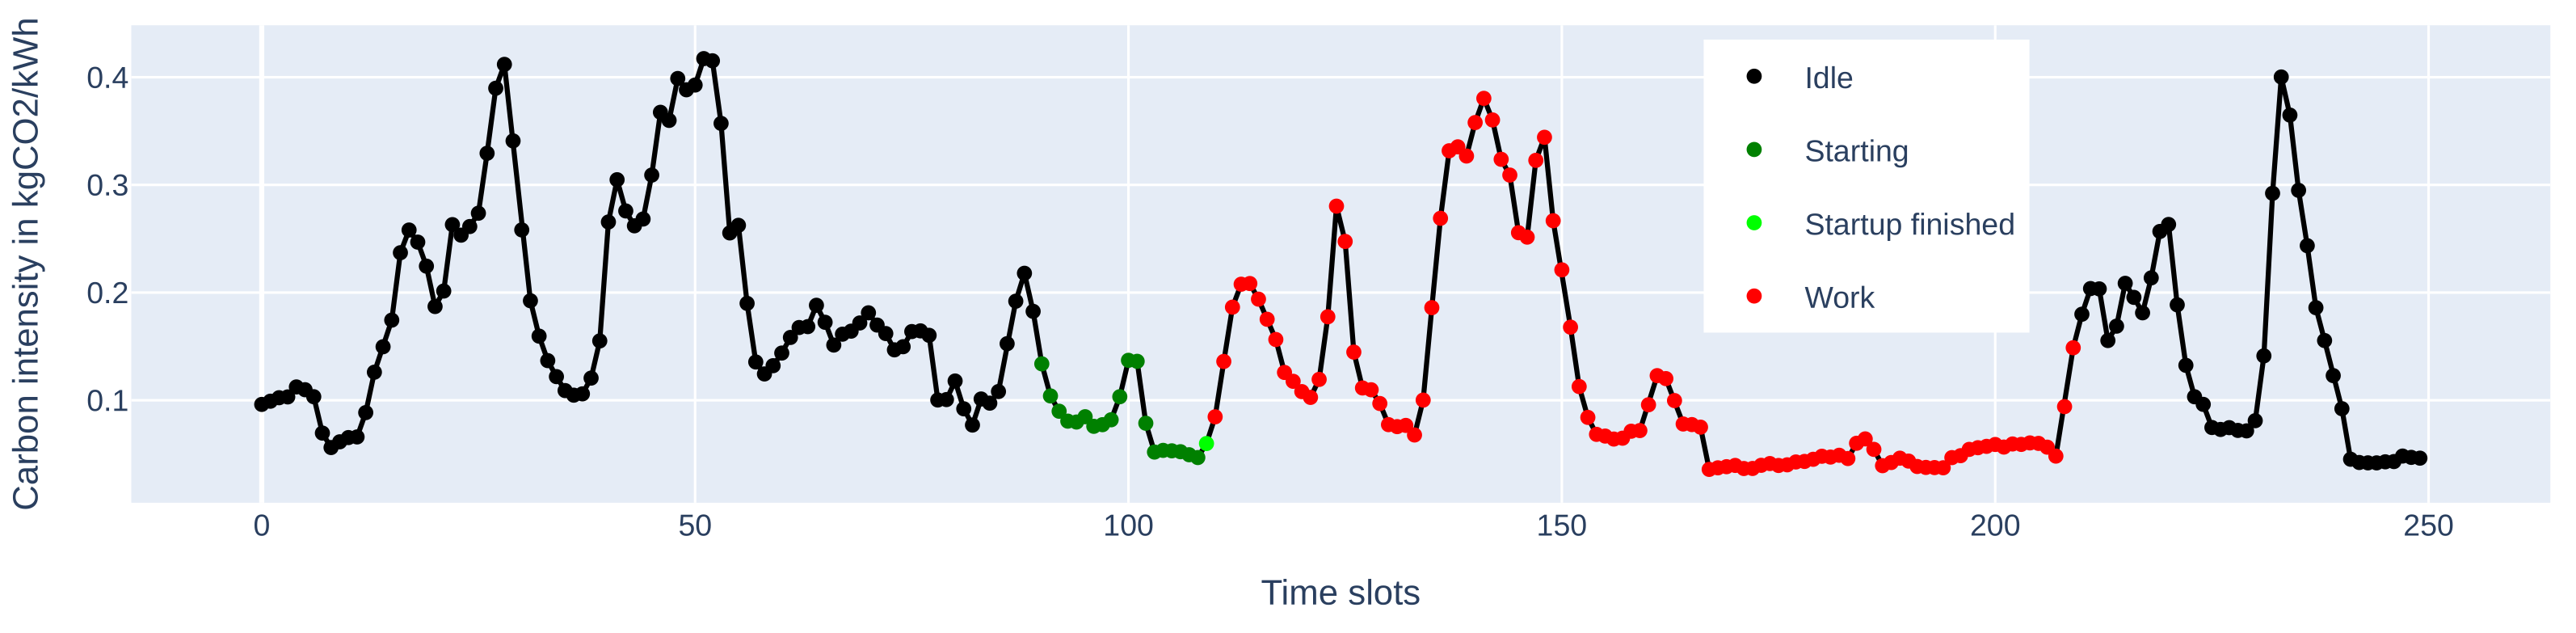
\includegraphics[width=\linewidth]{GAIA/notebooks/lp_overhead.pdf}
    \caption{The schedule of the second iteration. In addition to time slots being assigned for work, a startup phase must also be scheduled before work can begin. The light-green mark indicates a helper variable, used for this mechanic. In comparison to the previous figure, there is now one long, connected, block where the job is worked on, as resuming a job carries an extra cost.}
    \label{fig:lp_overhead}
\end{figure}

\paragraph{Adding a Notion of Progress}

So far, the assumption of constant power has been continued.
Changing this assumption under the previous scheduler using the greedy algorithm in section \ref{sec:uninterrupted_oracle_scheduling}, was relatively easy, as changing the constant expression to a Python function of the model sufficed. 
This cannot be reused in LP, however, as the problem definition may only include linear equations, which a generic function is not. 
To add dynamic power into the linear program, we decided to \emph{linearize} the function, meaning the model needed to be split up into multiple linear approximations.

As the model already is essentially a step function of time to power, each phase being one step, the mapping is inherently pretty close. 
As such, \emph{a lot} of equations were needed that each express "if the progress in the job is $t$, set power to $model(t)$". 
For that, a notion of progress and time is needed in the model.
The progress inside each startup-phase needs to reset, as that can happen multiple times during the schedule. 
On the other hand, the progress for the productive work must not be reset between execution blocks. 

We add the following code to express this:

\begin{minipage}{\linewidth}
\begin{lstlisting}[frame=single, numbers=left, caption={Progress Variables in LP}, label={list:lp_progress}, basicstyle=\ttfamily, breaklines]
# define "work_time_progressed" and "startup_time_progressed" as 
# DEADLINE-many integer variables

M = DEADLINE * 2
for t in range(DEADLINE-1):
    if (t>0):
        prob += startup_time_progressed[t] >= startup_time_progressed[t-1] + 1 - (1 - starting[t]) * M 
        prob += startup_time_progressed[t] <= startup_time_progressed[t-1] + 1 + (1 - starting[t]) * M
    prob += startup_time_progressed[t] <= starting[t] * M 
    prob += work_time_progressed[0] == 0
    if (t > 0):
        prob += work_time_progressed[t] == work_time_progressed[t-1] + work[t]
\end{lstlisting}
\end{minipage}

Basically, the idea is to count up each progress variables by 1, if a time slot is being determined for work or startup respectively (see line 12 for this).

This snippet also includes an LP "trick", namely the \emph{Big M Method}. 
In line 4, a constant \verb|M| is defined as "a \emph{large} integer, that cannot otherwise occur in the result set", , "large" being twice the amount of time slots, although it could also be any other arbitrarily chosen large number.

Take line 9 as an example: 
remember that \verb|starting[t]| is either $0$ or $1$, multiplying this by a large number means the right side is either $0$ or "\emph{large}". 
Constraining a variable to be less than \verb|M| effectively does nothing (is "\emph{relaxed}"), as every value of that variable is less than \verb|M| by definition of \verb|M|. 
On the whole, this can expression be translated to "if a time slot is not used for starting the job, set the progress to 0, otherwise ignore this constraint", the Big M Method enables a way to add conditional constraints to a model!

While line 9 defines the \verb|startup_progress| outside the startup phases, lines 7 and 8 are needed to increase the progress by exactly 1. 
Notice how depending on the type of inequality, \emph{M} is either added or subtracted to the equation, a conditional \emph{greater than} relation is relaxed by setting the constraint to zero.

All in all, there is now a way to keep track of a job's progress inside the model, as shown in Figure \ref{fig:lp_progress}'s upper graph. Attention should be drawn to the \verb|work_progress| which keeps its value even when time slots are set to idle. 
The schedule found by the solver is not different from the previous one which added overhead, as the optimization goal was not changed and the progress indicators have no impact on the scheduling (yet).

\begin{figure}
    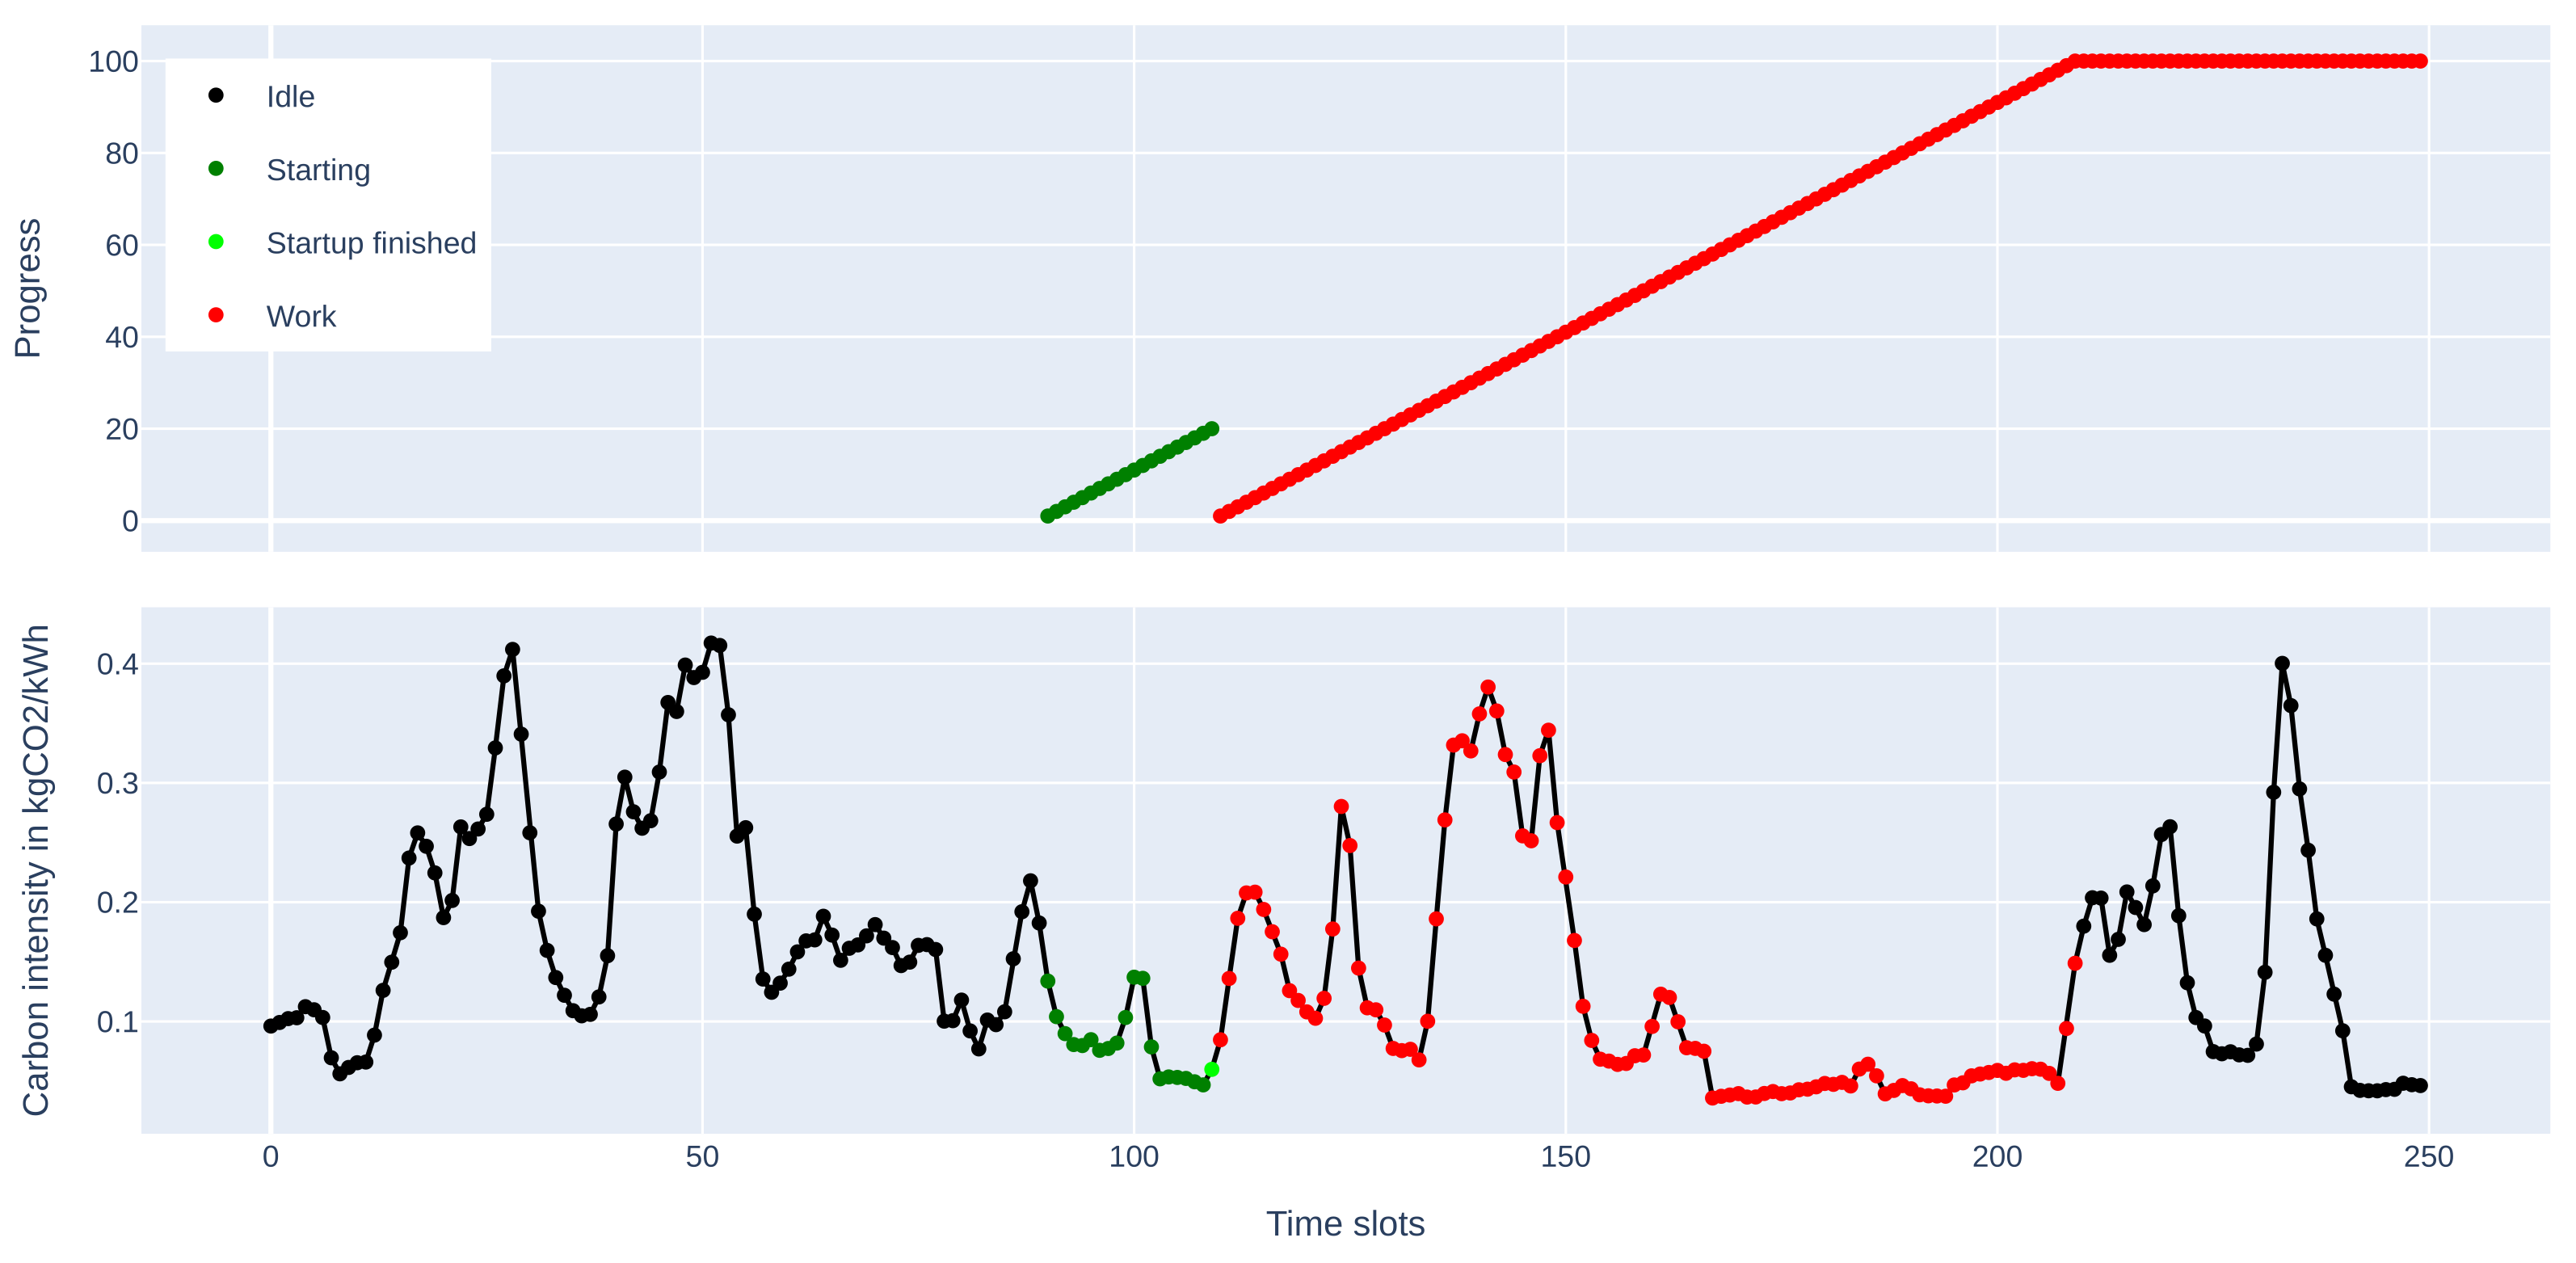
\includegraphics[width=\linewidth]{GAIA/notebooks/lp_progress.pdf}
    \caption{Visualisation of the result set after adding progress indicators. For either starting up or working, count up a respective integer variable. These do no yet impact the schedule itself, compared to Figure \ref{fig:lp_overhead}. Progress is kept even when idling.}
    \label{fig:lp_progress}
\end{figure}

\paragraph{Adding Power According to \modelname}

The goal of this part will be to have an LP variable for each phase, which indicates when the job is in that phase.
When such indicators exist, the formula for calculating a time slot's carbon emissions can be changed to Formula \ref{formula:total_carbon}:

\begin{align}
    \label{formula:total_carbon}
    carbonEmitted(t) = \sum_{p \in Phases} isActive(p, t) * powerOfPhase(p) * carbonEmission(t)
\end{align}

With that goal in mind, we add the pseudocode in Listing \ref{list:lp_phases} to determine when a phase is active. 

\begin{minipage}{\linewidth}
\begin{lstlisting}[frame=single, numbers=left, caption={Phase detection in LP}, label={list:lp_phases}, basicstyle=\ttfamily, breaklines]
# for each phase
# let phase_indicator, phase_indicator_upper, phase_indicator_lower be DEADLINE-many boolean variables
# set lower_bound to be the minimum progress this phase can occur in 
# set upper_bound to be the maximum similarly

# do the following for each phase
for t in range(DEADLINE):
    prob += progress[t] - lower_bound <= M*phase_indicator_lower[t]
    prob += lower_bound - progress[t] <= M*(1-phase_indicator_lower[t])

    prob += upper_bound - progress[t] <= M*phase_indicator_upper[t]
    prob += progress[t] - upper_bound <= M*(1-phase_indicator_upper[t])

    prob += phase_variable[t] >= phase_indicator_lower[t] + phase_indicator_upper[t] - 1
    prob += phase_variable[t] <= phase_indicator_lower[t]
    prob += phase_variable[t] <= phase_indicator_upper[t]
\end{lstlisting}
\end{minipage}

Unwrapping this, two helper variables are added per phase and each time slot. 
A lower variable indicates that the previously established progress is above the threshold for a phase, while the upper variable indicates the opposite. 
The \verb|phase_variabel| is then \emph{active} where these two overlap (lines 14 to 17 define a logical \emph{AND}).

The constraint of line 8 is only applied if the indicator is \verb|false|.
If it is false, the progress at the time slot must be below the lower bound (as negative numbers are equal to zero).
Line 9 works on the negated indicator, applying the constraint if it is \verb|true|. 
If the indicator is \verb|true|, progress must be higher than the lower bound. 
Combining this, the expression \verb|phase_indicator_lower[t] <=> progress[t] > lower_bound| is added to the model. 
The upper bound is formulated in the following two lines similarly.

Using this addition, the schedule now looks like the one shown in Figure \ref{fig:lp_states}. 
Unlike the previous times, splitting the job up into two parts is now the optimal solution. 
Attention should be drawn to the circumstance that the high-powered phase (the green one) is scheduled on the lowest carbon emissions while the low-powered one is scheduled on the higher emission time slots.

\begin{figure}
    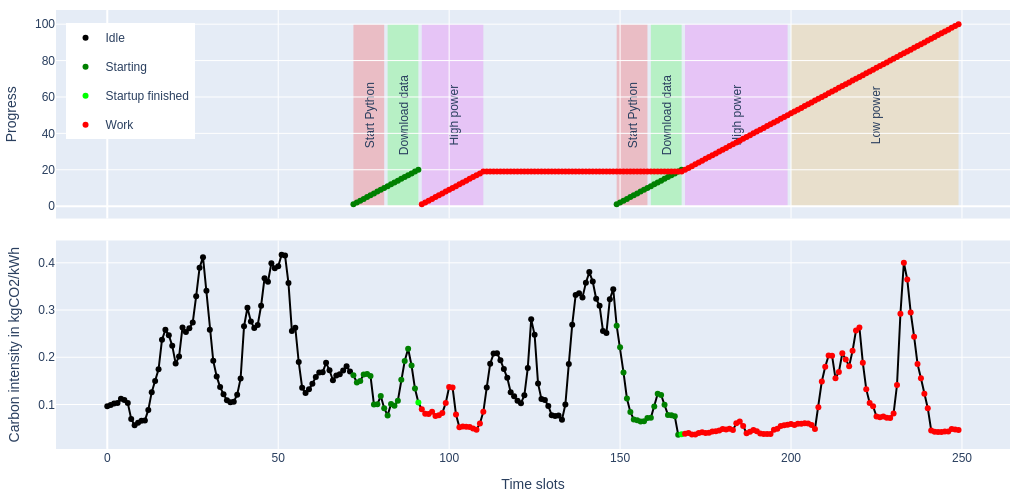
\includegraphics[width=\linewidth]{GAIA/notebooks/lp_states.pdf}
    \caption{The final scheduling including differing power levels according to phases. In this example, there is a high-powered phase at 230 W and a low powered phase at 100 W. Unlike before, it is now optimal to suspend \& resume the job to schedule the high-powered phase on the least carbon intensive time slots (170 to 200)}
    \label{fig:lp_states}
\end{figure}

\paragraph{Issues of the implementation}

As of now, checkpointing may happen at any point in the scheduler, as the \verb|work_progress| is never reset. 
Future work will focus on checkpointing at specific points, such as after specific phases like in the entry ML example in Section \ref{sec:future_work}.\todo{Add this to future work!}

Another issue at this point is the runtime and hardware requirements for finding a solution.
While the upper example of 250 time slots and a job length of 120 were found within minutes on a laptop\footnote{specifically, Lenovo T470 with 8 GB RAM and an i5-7200U CPU @ 2.50GHz}, bigger problem sizes such as 5000 time slots and a length of 800 barely finish within 30 minutes with a \emph{gap} value of 98\%.
The gap value is an indicator of how close the solver is to finding the optimal solution, with 0\% representing the optimal solution.

Solvers are able to take advantage of multiple CPU cores; however, in our case, the issue was likely a lack of memory. 
Glancing into the system monitor utility on Ubuntu then shows that all 8 GB of RAM are in use and that swap space is being utilized a lot.

\paragraph{Decreasing the Problem Size}

In the previously shown Figures, each carbon emission data point corresponds to one time slot, which in turn corresponds to one unit of time in the job. 
Going by the resolution of the carbon emissions, each data point describes the emissions for one hour. 
In the original \verb|GAIA| implementation, job lengths are given in seconds, however. 
The example workload used for measuring in Section \ref{sec:power_measurements} also showed that timescales in seconds are useful. 

Using a 1:1 mapping between those results in 3600 (60s * 60) time slots for each hour, resulting in very large problem sizes in turn needing long execution times and high amounts of memory.

In order to improve on the issues mentioned above, the following optimization is made: by calculating the \emph{greatest common divisor (gcd)} between all phase durations and the time resolution of the carbon emissions (3600), all durations can be scaled down by the \verb|gcd|. Each time slot in the model then represents \verb|gcd|-many seconds.

The effect of this optimization heavily depends on the input phases. 
If there are very short phases, the \verb|gcd| is low likewise, resulting in minimal reduction of the problem size.
